\documentclass{article}
\usepackage{tikz}
\usetikzlibrary{external}
\tikzexternalize[mode=list and make]

\tikzset{
    % Defines a custom style which generates BOTH, .pdf and .png export
    % but prefers the .png on inclusion.
    %
    % This style is not pre-defined, you may need to copy-paste and
    % adjust it.
    png export/.style={
        external/system call/.add={}{; convert -density 300 -transparent white "\image.pdf" "\image.png"},
        %
        /pgf/images/external info,
        /pgf/images/include external/.code={%
            \includegraphics
            [width=\pgfexternalwidth,height=\pgfexternalheight]
            {##1.png}%
        },
    },
    %
    png export,% ACTIVATE
}

\begin{document}

{
% Here we specify the figure will be converted and inserted as PNG
\tikzset{png export}
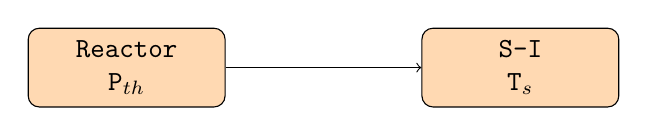
\begin{tikzpicture}[
    base/.style = {rectangle, rounded corners, draw=black,
minimum width=3cm, minimum height=1cm,
text centered, font=\sffamily},
process/.style = {base, minimum width=2.5cm, fill=orange!30,
font=\ttfamily},
node distance=3cm,
every node/.style={fill=white, font=\sffamily}, align=center
]

  \node (reactor) [process] {Reactor\\P$_{th}$};
  \node (si)     [process, right of=reactor, xshift=2.cm] {S-I\\T$_s$};
  
  \draw[->]     (reactor) -- (si);


\end{tikzpicture}
}

{
% Here we specify the figure will be converted and inserted as PNG
\tikzset{png export}
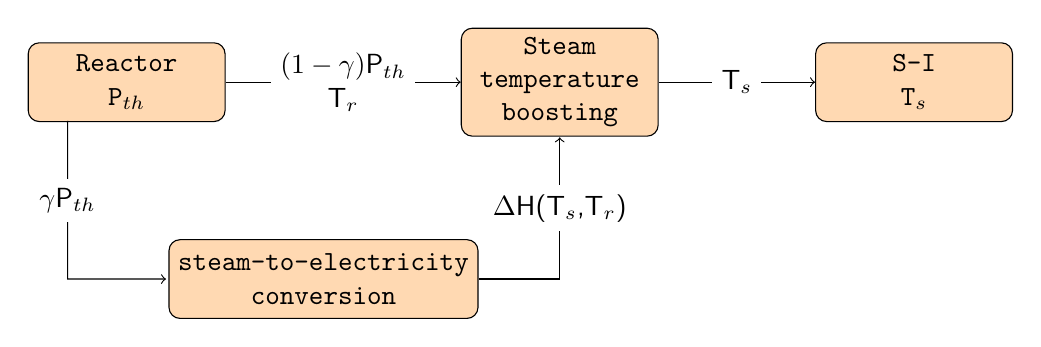
\begin{tikzpicture}[
    base/.style = {rectangle, rounded corners, draw=black,
minimum width=3cm, minimum height=1cm,
text centered, font=\sffamily},
process/.style = {base, minimum width=2.5cm, fill=orange!30,
font=\ttfamily},
node distance=3cm,
every node/.style={fill=white, font=\sffamily}, align=center
]

  \node (reactor) [process] {Reactor\\P$_{th}$};
  \node (steam1)   [process, below of=reactor, xshift=2.5cm, yshift=0.5cm] {steam-to-electricity\\conversion};
  \node (steam2)   [process, right of=reactor, xshift=2.5cm] {Steam\\temperature\\boosting};
  \node (si)      [process, right of=steam2, xshift=1.5cm] {S-I\\T$_s$};

  \draw[->]     (reactor) -- (steam2) node[midway] {$(1-\gamma)$P$_{th}$\\T$_r$};
  \draw[->]     (steam2) -- (si) node[midway] {T$_s$};
  \draw[->]     (reactor) -- ++ (-0.75,-0.5)-- node[midway] {$\gamma$P$_{th}$} ++ (0.,-2.)-- ++ (1.25,0);
  \draw[->]     (steam1) -- ++ (2,0.)-- ++ (1,0) -- node[midway] {$\Delta$H(T$_s$,T$_r$)} ++ (0.,1.8);

\end{tikzpicture}
}

\end{document}

% To compile do make; make -f hte1.makefile


